\section{Literature Survey} \label{literature_survey}

In this section I briefly describe some of the literature I surveyed
and considered important for our current and future work. I point out
some salient features and contributions of each of the papers listed.

%%%%%%%%%%%%%%%%%%%%%%%%%%%%%%%%%%%%%%%%%%%%%%%%%%%%%%%%%%%%%%%%%%%%%%%%%%%%%%%

\subsection{Initial exploration - EagleSense}
One of the first projects we explored as relevant to our project was
the work done by Wu et
al.~\cite{18b6b9f75d1645c0a1433a2ce7bfce0f}. They describe their
system(\emph{EagleSense}) which is a real-time tracking infrastructure
using top-view depth-sensors capable of detecting users' posture,
position, orientation and activity. In a scene where multiple people
interact with each other at the same time, conventional techniques,
that use front facing cameras, suffer from the problem of
occlusions. Top-view camera-based tracking avoids this problem of occlusion.

Here are some of the highlights of this work (which also happen to be
very desirable for our intended work):

\begin{enumerate}
\item \textbf{Non-invasive tracking}: Users don't have to wear markers
\item \textbf{Off-the-shelf technology}: Uses Kinect. While a device
  like Walabot is not completely off-the-shelf (as in easily
  commercially available) at the time of this writing, it is a very
  affordable device.
\item \textbf{Reliability}: Realtime updates with minimal delays.
\item \textbf{High-level access to spacial data}: Easy access to
  realtime data
\item \textbf{Configurability for activities}: For extensibility.
\end{enumerate}

%%%%%%%%%%%%%%%%%%%%%%%%%%%%%%%%%%%%%%%%%%%%%%%%%%%%%%%%%%%%%%%%%%%%%%%%%%%%%%%

\subsection{Nonverbal communication analysis}
Although a bit outdated, a good starting point was the review work
done by Gatica et
al.~\cite{Gatica-Perez:2009:ANA:1621144.1621313}. The paper reviews
state of the art research in the field of human interaction study as
of 2009. In this paper, the authors lay out the importance of non
verbal aspect of comunication such as body gestures, posture, eye gaze
and facial expressions along with spoken words.

Here is a highlight of their focus:

\begin{enumerate}
  \item The main focus of this paper is \emph{focus on nonverbal behavior}
  \item The authors quote Hall et al,. \emph{``specific non-verbal behaviors
    often cannot be mapped onto specific meanings with any
    certainty''}~\cite{Hall2015}. Owing to this fact, they claim that
    the work in this field has a strong trial-and error type of
    empirical flavor.
  \item The paper mainly focusses on interaction among participants in
    small groups and cite references that show that small groups are
    more dynamic than larger groups.
  \item Studies face-to-face conversations of physically collocated
    groups of people.
  \item They focus on social constructs by extracting features from
    audio/video and talks about computational models
  \item They discuss \emph{model interaction management} and elaborate
    on two aspects of it namely \emph{addressing} (to whom the speech
    is directed) and \emph{turn-taking behavior}.
\end{enumerate}

I consider identifying and tracking behavior in groups as very
important to our project as it is likely to be a key component of
activity tracking.

%%%%%%%%%%%%%%%%%%%%%%%%%%%%%%%%%%%%%%%%%%%%%%%%%%%%%%%%%%%%%%%%%%%%%%%%%%%%%%%

\subsection{Cross-Device Interaction}

Similar to the EagleSense work, another paper that hit close to home
was the work done by Marquardt et
al.~\cite{Marquardt:2012:CIV:2380116.2380121}. They built a system
called \emph{GroupTogether} that explores corss-device interaction
using two socialogical constructs: \emph{F-formations} and
\emph{micro-mobility}.

Salient features of this work were:

\begin{itemize}
\item The hardware included, a pair of overhead kinect depth cameras,
  low-power 8GHZ band radio modules and accelerometers to detect tilting
  of slate devices.
\item study of F-formations (discussed in detail in a forthcoming
  section)
\item \emph{micro-mobility}: orientation and repositioning of objects
  so that they may be fully or partially viewed or concealed from
  other persons.
\item they study proxemics of people as well as proxemics of devices
\item they make a case that human conversation is fluid and dynamic but,
  discussions that rely on digital content remains stiff and
  unnatural because manipulating, sharing and displaying
  information on and across multiple devices is cumbersome.
\item Physically nearby people in the r-space expecially those
  facing away are recognized as socially distinct and therefore
  can be excluded from the exchange.
\item In this system, if people \emph{within} the F-formation orient
  their devices towards the central o-space the system offers
  lightweight ways to share device contents accross the group.
\end{itemize}

While I certainly subscribe to the ideas proposed in this paper, their
experiments were on videos of interacting people. They do not address
occlusions. The paper also does not carry out these detections on live
data. Nevertheless, the fact that they heavily involve devices and
track the humans interacting with devices, there is definitely lessons
to be learned here. Building upon this work and data from our 3D
sensors, we should attempt to go from activity detection (as done in
this paper) to human group dynamics and activity tracking.

%%%%%%%%%%%%%%%%%%%%%%%%%%%%%%%%%%%%%%%%%%%%%%%%%%%%%%%%%%%%%%%%%%%%%%%%%%%%%%%

%% verbatim
\subsection{Gestures \& Proxemics}
For a better understanding into the social aspects of human
interaction and social behavior, I briefly surveyed the works by
Edward T. Hall and Adam Kendon.

In \emph{From gesture in conversation to visible action as
  utterance}\cite{bec44a41-d3b1-44f3-848a-aab268493c14} the authors
mention the work by Adam Kendon, in the field of \emph{Gesture
  Studies}. The field of gesture study of how bodily movements are
associated with one's speech.

Hall~\cite{Hall-1990} defines \emph{proxemics} as the study of
\emph{``observations and theories of man's use of space''}. The
sociological field of proxemics studies people's use of personal space
to mediate social interations. The defining characterstic is that
people equate interpersonal physical distance with social distance. He
also describes social zones basedon phusical distance bewteen people,
ranging from intimate (0-50cm), personal (1m) social (4m) and public
(> 4m).

The implication of this fact is that proximity becomes a very of
people's desire to communicate with another participant via the
devices they carry.

%%%%%%%%%%%%%%%%%%%%%%%%%%%%%%%%%%%%%%%%%%%%%%%%%%%%%%%%%%%%%%%%%%%%%%%%%%%%%%%

\subsection{Study of F-Formations}
Most of the literature that I looked at had made use of the concept of
F-formations. It stands for \emph{Facing Formation}.  ``F-formation is
a social-spatial formation in which people have established and
maintain a convex space (called \emph{o-space}) to which everybody in
the gathering has direct, easy and equal access''. People arrange
themselves in circle, ellipse, horseshoe, side-by-side or L-shape so
that can have easy and preferential access to members of the group.

One of the first milestones of the project is to be able to firstly
identify such groups and then correctly label them based on their
shape and orientations.

The pioneer researcher Adam Kendon~\cite{Kendon:formation:1990}
defines the term as, \emph{``an F-formation arises whenever two or
  more people sustain a spatial and orientational relationship in
  which the space between them is one to which they have equal,
  direct, and exclusive access''}. Less formally, it is a study that
deals with how people orient themselves in each of the three social
spaces namely: \emph{o-space}, \emph{p-space} and \emph{r-space}. It
specifically deals with physical arrangements that people adopt during
focussed encounters. In an interacting group, o-space is the space
that can be considered inside the circle or refers to the inner area
that is enclosed by the people in the group. The p-space is the narrow
layer that holds the people. Outside of these two spaces is the
r-space.

\begin{figure}[H]
  \begin{center}
    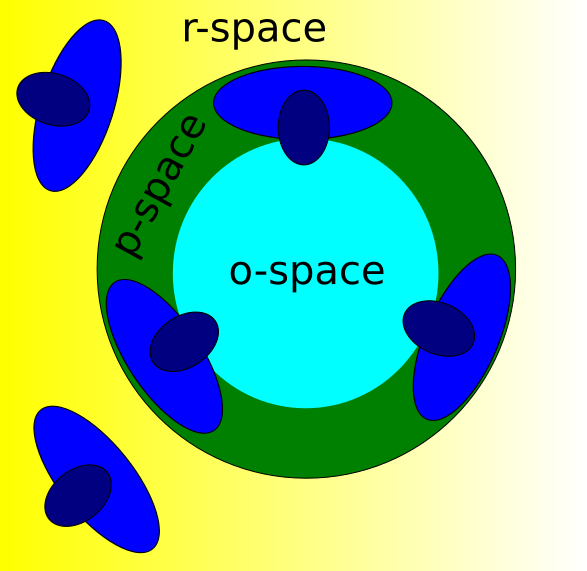
\includegraphics[scale=.45]{figures/o-p-r-space}
    \caption{A pictorial representation of people in F-formation and a
      description of the various components}
    \label{fig:f-formation}
  \end{center}
\end{figure}

%%%%%%%%%%%%%%%%%%%%%%%%%%%%%%%%%%%%%%%%%%%%%%%%%%%%%%%%%%%%%%%%%%%%%%%%%%%%%%%
\subsection{Social interaction discovery, group detection \& tracking}

Cristani et al.,~\cite{DBLP:conf/bmvc/CristaniBPFTBMM11} did
pioneering work in F-formation detection using statistical
techniques. The authors describe a novel way of detecting F-formations
using \emph{Hough transform}~\cite{Duda:1972:UHT:361237.361242}. In
conclusion they state that using temporal information it might be
possible to more reliable detection. They further go on to say that if
one could extract additional features from the detected F-formations,
it might be possible to predict and understand social interactions and
situations.

%%%%%%%%%%%%%%%%%%%%%%%%%%%%%%%%%%%%%%%%%%%%%%%%%%%%%%%%%%%%%%%%%%%%%%%%%%%%%%%

\subsubsection{Group detection}
In a series of work by Setti et al.~\cite{6616147,6738732}, they
mention their efforts for group detection. They describe F-formation
as a loose geometric arrangement of people and offer two distinct
methods of detecting groups. These methods are \emph{Hough
  voting}~\cite{Duda:1972:UHT:361237.361242} and graph
theory~\cite{Hung:2011:DFD:2070481.2070525}. The paper concludes that
Hough voting approach performs better using people's position and
orientation which robustness to noise. The graph theoritical technique
(or Dominant Sets for F-Formation(DSFF)) performs better when only one
position information is available. As a result of this work they
identified groups of conversing people.

In a more recent paper titled \emph{F-formation Detection:
  Individuating Free-standing Conversational Groups in Images}, the
authors~\cite{DBLP:journals/corr/SettiRBC14} introduce a new method
called \emph{Graph-Cuts for F-formation}(GCFF) for automatic of
detection of groups in still images using
\emph{graph-cuts}~\cite{greig1989exact}. They study free standing
conversational groups.

It is handy to be aware of a multitude of such techniques while
performing an activity like group tracking. This will reduce the
number of moving parts in our experiments. This is important because
our data sources are not the same as the ones used in these
experiments which already introduces a different kind of variability.

%%%%%%%%%%%%%%%%%%%%%%%%%%%%%%%%%%%%%%%%%%%%%%%%%%%%%%%%%%%%%%%%%%%%%%%%%%%%%%%

\subsubsection{Group tracking}
Bazzani et al.,~\cite{6247888} talk about tracking groups of people in
surveillance scenarios. They make use of a technique called
\emph{Decentralized Particle Filter(DPF)}~\cite{5629376}. They show the
relation between modeling of individuals and of groups and further
demonstrate that groups are better tracked if individuals are
considered and viceversa.

Given that the authors have successfully demonstated the utility of a
customized version of DPF, I would consider it a highly useful tool to
keep in our back pocket as this subject will surface in our study
group activity tracking.

%%%%%%%%%%%%%%%%%%%%%%%%%%%%%%%%%%%%%%%%%%%%%%%%%%%%%%%%%%%%%%%%%%%%%%%%%%%%%%%

\subsection{Constraints from physical structures}

Marshall~\cite{Marshall:2011:UFA:1958824.1958893} studied social
interactions between visitors and staff in a tourist information
center. They particularly looked at interactions across counters. The
authors used F-formations as a basis to show how some features in
physical environment discourage the creation of F-formation thereby
discouraging certain types of interactions.

Results from this paper are particularly important to us and will be
of significance when we are trying to predict dynamic behavior of
group participants.
%%%%%%%%%%%%%%%%%%%%%%%%%%%%%%%%%%%%%%%%%%%%%%%%%%%%%%%%%%%%%%%%%%%%%%%%%%%%%%%
